\documentclass[mathserif,11pt]{beamer}

\usecolortheme[RGB={55,110,144}]{structure} % prima c'era questo bluetto: 20,104,204  % blu elettrico: 20,10,244


\usepackage{bbm,color,xcolor}
\usepackage{colortbl}
\usepackage{animate}
\usepackage[utf8]{inputenc}
\usepackage{verbatim}
\usepackage{eulervm}
\usepackage{fontenc}
\usepackage{xmpmulti}
\usepackage[absolute,overlay]{textpos}
\usepackage{pifont}
\usepackage{default,amsmath,comment,amssymb,amsthm,amscd,latexsym,tcolorbox,array}
\usepackage{amsfonts,mathrsfs,nomencl,hyperref,threeparttable,textcomp}
\usepackage[english]{babel}
\usepackage{graphicx}
\usepackage{tabularx,tikz,pgfplots,setspace,subfigure,epigraph,lscape,color,booktabs,multirow}
\usepackage{fancybox,changes,pgfpages,array, booktabs}
\usepackage{pgfplots}
\usepackage{times}
\usepackage[labelformat=empty,labelsep=none]{caption}
\usepackage{bm}
 \usepackage{enumitem}



\def\darkred{\color{red!50!black}}
\def\darkgreen{\color{green!50!black}}
\def\darkblue{\color{blue!50!black}}
\definecolor{mycolor}{rgb}{0.28,0.69,0.7}
\definecolor{mycolor1}{rgb}{0.7,0.75,0.71}
\definecolor{mycolor2}{rgb}{0.58,1,1}
\definecolor{darkred}{rgb}{0.5,0,0}
\definecolor{lightred}{rgb}{1,0.5,0.5}
\definecolor{lightblue}{rgb}{0.7,0.7,1}
\definecolor{magenta1}{cmyk}{0.1,0.8,0.3,0.1}
\definecolor{magenta2}{cmyk}{0.1,0.8,1,0.1}
\definecolor{magenta3}{cmyk}{0.2,0.9,1,0.1}
\definecolor{magenta4}{cmyk}{0.3,0.7,1,0.1}
\definecolor{cdef}{rgb}{0,0,0.5}
\definecolor{cdef2}{rgb}{0,0,0.8}
\definecolor{cdef3}{rgb}{0.5,0,0.3}
\definecolor{cemph}{rgb}{0,0.5,0}
\definecolor{mycolor}{rgb}{0.9,0.04,0.02}  
\definecolor{mydarkblue}{rgb}{0,0.08,0.45}  
\definecolor{col0}{rgb}{0.000,0.000,0.000}
\definecolor{col1}{rgb}{0.000,0.000,1.000}
\definecolor{col2}{rgb}{0.000,1.000,0.000}
\definecolor{col3}{rgb}{0.000,1.000,1.000}
\definecolor{col4}{rgb}{1.000,0.000,0.000}
\definecolor{col5}{rgb}{1.000,0.000,1.000}
\definecolor{Yellow}{rgb}{1.000,1.000,0.000}
\definecolor{col7}{rgb}{1.000,1.000,1.000}
\definecolor{Darkblue}{rgb}{0.000,0.000,0.560}
\definecolor{Blue}{rgb}{0.000,0.000,0.690}
\definecolor{Lightblue}{rgb}{0.000,0.000,0.820}
\definecolor{darkgreen}{rgb}{0.000,0.560,0.000}
\definecolor{Green}{rgb}{0.000,0.690,0.000}
\definecolor{LightGreen}{rgb}{0.000,0.820,0.000}
\definecolor{Turquoise}{rgb}{0.000,0.560,0.560}
\definecolor{Aquamarine}{rgb}{0.000,0.690,0.690}
\definecolor{col17}{rgb}{0.000,0.820,0.820}
\definecolor{RedViolet}{rgb}{0.560,0.000,0.000}
\definecolor{RubineRed}{rgb}{0.690,0.000,0.000}
\definecolor{WildStrawberry}{rgb}{0.820,0.000,0.000}
\definecolor{Violet}{rgb}{0.560,0.000,0.560}
\definecolor{col22}{rgb}{0.690,0.000,0.690}
\definecolor{col23}{rgb}{0.820,0.000,0.820}
\definecolor{Brown}{rgb}{0.500,0.190,0.000}
\definecolor{col25}{rgb}{0.630,0.250,0.000}
\definecolor{Bitter}{rgb}{0.750,0.380,0.000}
\definecolor{Pink}{rgb}{1.000,0.000,1.00}
\definecolor{col28}{rgb}{1.000,0.630,0.630}
\definecolor{col29}{rgb}{1.000,0.750,0.750}
\definecolor{col30}{rgb}{1.000,0.880,0.880}
\definecolor{Dandelion}{rgb}{1.000,0.840,0.000}
\definecolor{_darkblue}{rgb}{0,0.01,0.75}  
\definecolor{_cdef}{rgb}{0.75,0.38,0}
\definecolor{_cdef1}{rgb}{0.95,0.88,0.6}
\definecolor{_lightgrey}{rgb}{0.9,0.9,0.9}
\definecolor{VeryLightBlue}{rgb}{0.830,0.810,1.000}

\def\dlb#1{\textcolor{VeryLightBlue}{#1}}
\def\db#1{\textcolor{_darkblue}{#1}}
\def\rfl#1{\dlb{[{\sf \scriptsize #1}]}}
\def\rf#1{\db{[{\sf \scriptsize #1}]}}
\def\txtl#1{\textcolor{_lightgrey}{#1}}
\def\koml#1{\dlb{{\bf \small #1}}}
\def\kom#1{\db{{\bf \small #1}}}
\def\rkl#1{\cde1f{{\bf \small #1}}}
\def\rk#1{\cdef{{\bf \small #1}}}
\def\cdef#1{\textcolor{_cdef}{#1}}
\def\cde1f#1{\textcolor{_cdef1}{#1}}
\newcommand{\blue}[1]{\textcolor{_darkblue}{#1}}
\newcommand{\red}[1]{\textcolor{col4}{#1}}
\newcommand{\cd}[1]{\textcolor{_cdef}{#1}}

%% Fond blanc, titre en red 

\newcommand{\mythm}[2]{
  \begin{tcolorbox}[colframe=blue!75!black,colback=white,title={\sf\small #1}]
#2
\end{tcolorbox}
}


\renewcommand{\familydefault}{\rmdefault}
\newcommand{\MySingleArrow}[2][]{\tikz[baseline] \node [My Arrow Style,#1] {#2};}
\newcommand{\semitransp}[2][35]{\color{black!#1}#2}


\usetikzlibrary{fit}
\usetikzlibrary{calc}
\usetikzlibrary{plotmarks}
\usetikzlibrary{matrix}
\usetikzlibrary{positioning}
\usetikzlibrary{mindmap,backgrounds}
\tcbuselibrary{listings,breakable,skins}
\usetikzlibrary{arrows,shapes}
\usetikzlibrary{shapes.geometric}
\usetikzlibrary{trees}
\tikzset{My Double Arrow Style/.style={double arrow, fill=gray!50, anchor=base, align=center,text width=1.0cm}}
\tikzset{My Arrow Style/.style={single arrow, fill=gray!50, anchor=base, align=center,text width=2.8cm}}
\tikzset{
 treenode/.style = {align=center, inner sep=4pt, text centered,
    font=\sffamily},
  arn_n/.style = {treenode, rounded corners, rectangle, black, font=\sffamily, draw=black,minimum height=2em,
    fill=white}, 
leaf/.style = {treenode, rectangle, draw=black,
    minimum width=1em, minimum height=1em}
}
\tikzset{box1/.style={draw=black, thick, rectangle,rounded corners, fill=black!7!white}}
\tikzset{box2/.style={draw=black, thick, rectangle,rounded corners, fill=black!7!white, minimum height=3cm}}
\newcommand{\MyDoubleArrow}[2][]{\tikz[baseline] \node [My Double Arrow Style,#1] {#2};}

\usetheme{default}
\setbeamerfont{page number in head/foot}{size=\large}
\setbeamertemplate{footline}[frame number]
\setbeamercolor{upcol}{fg=black,bg=green}      %\setbeamercolor{upcol}{fg=black,bg=orange} prima c'era questo
\setbeamercolor{lowcol}{fg=black,bg=green!40}  %\setbeamercolor{lowcol}{fg=black,bg=orange!40}
\setbeamertemplate{navigation symbols}{}
\setbeamertemplate{itemize items}[circle]

\setbeamerfont{frametitle}{size=\large}
\setbeamertemplate{frametitle}
{
  \vspace{2mm}
\begin{tcolorbox}[colback=green!5,colframe=blue!40!black,height=10mm]
{{\bf    \insertframetitle}}
\end{tcolorbox}

}


\setitemize{label=\usebeamerfont*{itemize item}%
  \usebeamercolor[fg]{itemize item}%
  \usebeamertemplate{itemize item}}

\DeclareBoldMathCommand{\bell}{\ell}
\DeclareBoldMathCommand{\bu}{u}
\DeclareBoldMathCommand{\bF}{F}
\DeclareBoldMathCommand{\bH}{H}
\DeclareBoldMathCommand{\bv}{v}
\DeclareBoldMathCommand{\bX}{X}
\DeclareBoldMathCommand{\bx}{x}
\DeclareBoldMathCommand{\bh}{h}
\DeclareBoldMathCommand{\bbf}{f}
\DeclareBoldMathCommand{\bb}{b}
\DeclareBoldMathCommand{\balpha}{\alpha}
\DeclareBoldMathCommand{\bbeta}{\beta}

\def\mF{\bF}
\def\mH{\bH}

\def\N{\mathbb{N}}
\def\K{\mathbb{K}}
\def\Kbar{\overline{\mathbb{K}}}
\def\Z{\mathbb{Z}}
\def\Q{\mathbb{Q}}
\def\M{\mathsf{M}}

\def\rank{\text{rank}}
\def\softO{\ensuremath{O{\,\tilde{ }\,}}}

\title[]{\huge \bf Homotopy techniques for \\ determinantal systems}
\author[]{
{\bf \'Eric Schost} \\ \vspace{0.1cm} University of Waterloo \\ \medskip
joint work with \\ \vspace{0.1cm} Jonathan Hauenstein, Mohab Safey El Din, {\bf Xuan Thi Vu}
}
\date{}

\begin{document}

%%%%%%%%%%%%%%%%%%%%%%%%%%%%%%%%%%%%%%%%%%%%%%%%%%%%%%%%%%%%
%%%%%%%%%%%%%%%%%%%%%%%%%%%%%%%%%%%%%%%%%%%%%%%%%%%%%%%%%%%%
%%%%%%%%%%%%%%%%%%%%%%%%%%%%%%%%%%%%%%%%%%%%%%%%%%%%%%%%%%%%

\begin{frame}

\maketitle

\end{frame}

%%%%%%%%%%%%%%%%%%%%%%%%%%%%%%%%%%%%%%%%%%%%%%%%%%%%%%%%%%%%
%%%%%%%%%%%%%%%%%%%%%%%%%%%%%%%%%%%%%%%%%%%%%%%%%%%%%%%%%%%%
%%%%%%%%%%%%%%%%%%%%%%%%%%%%%%%%%%%%%%%%%%%%%%%%%%%%%%%%%%%%

\begin{frame}

\frametitle{An example}

\rk{Goal:} minimize $X_1$ on $S: \red{X_1^{100}+ X_2^{100}+X_3^{100}=1}$.

\bigskip

The minima satisfy 
$$X_1^{100}+ X_2^{100}+X_3^{100}=1$$
and
$$
\rank  \begin{bmatrix}
100 X_1^{99} &  100 X_2^{99} &  100X_3^{99} \\
1 & 0 & 0
\end{bmatrix}
 < 2
$$

\bigskip

\rk{Optimization, real algebraic geometry (polar varieties), \dots}

\end{frame}

%%%%%%%%%%%%%%%%%%%%%%%%%%%%%%%%%%%%%%%%%%%%%%%%%%%%%%%%%%%%
%%%%%%%%%%%%%%%%%%%%%%%%%%%%%%%%%%%%%%%%%%%%%%%%%%%%%%%%%%%%
%%%%%%%%%%%%%%%%%%%%%%%%%%%%%%%%%%%%%%%%%%%%%%%%%%%%%%%%%%%%

\begin{frame}

\frametitle{Our problem}

\mythm{}{
  $\K$ is a field of characteristic zero.

  \smallskip

  Given
  \begin{itemize}
  \item a matrix $\mF \in \K[X_1,\dots,X_n]^{p \times q}$
  \item polynomials $G=(g_1,\dots,g_s)$ in $\K[X_1,\dots,X_n]$,
  \end{itemize}
  such that 
  $$p \leq q \quad\text{and}\quad n = q-p+s+1,$$ 
  compute the \only<1>{set}\only<2>{\rk{isolated points of} the set}
  $$\{\bx \in \Kbar{}^n \mid G(\bx)=0,\ \rank(\mF(\bx))<p\}$$
}

\end{frame}

%%%%%%%%%%%%%%%%%%%%%%%%%%%%%%%%%%%%%%%%%%%%%%%%%%%%%%%%%%%%
%%%%%%%%%%%%%%%%%%%%%%%%%%%%%%%%%%%%%%%%%%%%%%%%%%%%%%%%%%%%
%%%%%%%%%%%%%%%%%%%%%%%%%%%%%%%%%%%%%%%%%%%%%%%%%%%%%%%%%%%%

\begin{frame}

\frametitle{Why take \red{$n = q-p+s+1$}?}

This is because of known syzygies between minors.

\medskip

\begin{overlayarea}{\linewidth}{14\baselineskip}
\only<1>{
Suppose $s=0$, so \red{$n = q-p+1$}. 

\medskip

\mythm{Example (generic matrix)}{
$$\mF = \begin{bmatrix}
f_{1,1} & f_{1,2} & f_{1,3} \\
f_{2,1} & f_{2,2} & f_{2,3} 
\end{bmatrix}, \quad p = 2, \quad q=3$$
One syzygy:
{\small
\[f_{1,1} \red{(f_{1,2}f_{2,3}-f_{1,3}f_{2,2})}
- f_{1,2} \red{(f_{1,1}f_{2,3}-f_{1,3}f_{2,1})}
+ f_{1,3} \red{(f_{1,1}f_{2,2}-f_{1,2}f_{2,1})} =0
\]}
so if $\red{f_{1,1}\ne 0}$, only $\red{2}$ equations (with no further
relations)
}

\medskip

In general: localize with top-left \red{$(p-1)$}-minor, $\red{q-(p-1)}$ equations
}
\only<2>{

\mythm{Fact [Macaulay, Eagon-Northcott]}{
All irreducible components of the algebraic set
  $$\{\bx \in \Kbar{}^n \mid \rank(\mF(\bx))<p\}$$
have dimension at least $n-(q-p+1)$
}
}

\only<3>{
\mythm{Fact [Macaulay, Eagon-Northcott]}{
All irreducible components of the algebraic set
  $$\{\bx \in \Kbar{}^n \mid G(\bx)=0,\ \rank(\mF(\bx))<p\}$$
have dimension at least $n-(q-p+s+1)$
}
}
\end{overlayarea}

\end{frame}


%%%%%%%%%%%%%%%%%%%%%%%%%%%%%%%%%%%%%%%%%%%%%%%%%%%%%%%%%%%%
%%%%%%%%%%%%%%%%%%%%%%%%%%%%%%%%%%%%%%%%%%%%%%%%%%%%%%%%%%%%
%%%%%%%%%%%%%%%%%%%%%%%%%%%%%%%%%%%%%%%%%%%%%%%%%%%%%%%%%%%%

\begin{frame}

\frametitle{Main result -- column degrees}

\rk{Suppose that:}
\begin{itemize}
\item $n = q-p+s+1$
\item the degrees of $G=(g_1,\dots,g_s)$ are at most \blue{$\gamma_1,\dots,\gamma_s$},
\item the column-degrees of $\mF$ are at most \blue{$\alpha_1,\dots,\alpha_q$}
\item all polynomials are given by a SLP of size \blue{$L$}
\end{itemize}

\bigskip

\begin{overlayarea}{\linewidth}{14\baselineskip}

\only<1>{
\mythm{Theorem}{
\begin{itemize}[leftmargin=0.7em]
\item there are at most
  \begin{align*}
  \red{c= \gamma_1 \cdots \gamma_s E_{n-s}(\alpha_1,\dots,\alpha_q)}  
  \end{align*}
   \noindent isolated 
  solutions, counted with multiplicities 

\rk{($E_k$ = $k$-th elementary symmetric function)}

\item  can be computed  in time 
 $\red{(c L)^{O(1)}}$ (randomized algorithm)
\end{itemize}
}
}
\only<2>{
\mythm{Example}{
$$\mF = \begin{bmatrix}
    [2] & [1] & [5] & [7] \\
    [2] & [1] & [5] & [7] \\
    [2] & [1] & [5] & [7] 
  \end{bmatrix} \quad p=3, q=4, s=0 \implies \red{n=2}$$
  $c=E_2(2,1,5,7) = 2\cdot1+2\cdot5+2\cdot7+1\cdot5+1\cdot7+5\cdot7 = \red{73}$
}
}
\end{overlayarea}
\end{frame}

%%%%%%%%%%%%%%%%%%%%%%%%%%%%%%%%%%%%%%%%%%%%%%%%%%%%%%%%%%%%
%%%%%%%%%%%%%%%%%%%%%%%%%%%%%%%%%%%%%%%%%%%%%%%%%%%%%%%%%%%%
%%%%%%%%%%%%%%%%%%%%%%%%%%%%%%%%%%%%%%%%%%%%%%%%%%%%%%%%%%%%

\begin{frame}

\frametitle{Main result -- row degrees}

\rk{Suppose that:}
\begin{itemize}
\item $n = q-p+s+1$
\item the degrees of $G=(g_1,\dots,g_s)$ are at most \blue{$\gamma_1,\dots,\gamma_s$},
\item the row-degrees of $\mF$ are at most \blue{$\beta_1,\dots,\beta_p$}
\item all polynomials are given by a SLP of size \blue{$L$}
\end{itemize}

\bigskip

\begin{overlayarea}{\linewidth}{14\baselineskip}

\only<1>{
\mythm{Theorem}{
\begin{itemize}[leftmargin=0.7em]
\item there are at most
  \begin{align*}
  \red{c'= \gamma_1 \cdots \gamma_s S_{n-s}(\beta_1,\dots,\beta_p)}  
  \end{align*}
   \noindent isolated 
  solutions, counted with multiplicities 

\rk{($S_k$ = $k$-th complete symmetric function)}

\item  can be computed  in time 
 $\red{(c' L)^{O(1)}}$ (randomized algorithm)
\end{itemize}
}
}
\only<2>{
\mythm{Example}{
$$\mF = \begin{bmatrix}
    [2] & [2] & [2] & [2] \\
    [1] & [1] & [1] & [1] \\
    [5] & [5] & [5] & [5] 
  \end{bmatrix} \quad p=3, q=4, s=0 \implies \red{n=2}$$
$c'=S_2(2,1,5) = 2^2+2\cdot 1 + 2\cdot 5 + 1^2 + 1 \cdot 5 + 5^2 = \red{47}$
}
}
\end{overlayarea}
\end{frame}

%%%%%%%%%%%%%%%%%%%%%%%%%%%%%%%%%%%%%%%%%%%%%%%%%%%%%%%%%%%%
%%%%%%%%%%%%%%%%%%%%%%%%%%%%%%%%%%%%%%%%%%%%%%%%%%%%%%%%%%%%
%%%%%%%%%%%%%%%%%%%%%%%%%%%%%%%%%%%%%%%%%%%%%%%%%%%%%%%%%%%%

\begin{frame}

\frametitle{Previous work}

\rf{Giambelli} (see also~\rf{Miller-Sturmfels})
\begin{itemize}
\item Hilbert function of determinantal ideals of generic matrices
\item more refined type of degrees
\end{itemize}

\medskip

\rf{Nie-Ranestad}
\begin{itemize}
\item degree bounds $E_{n-s}(\cdots)$ and $S_{n-s}(\cdots)$ sharp for generic polynomials 
 (we reuse their construction for column degrees)
\end{itemize}

\medskip

\rf{Faug\`ere-Safey El Din-Spaenlehauer}, \rf{Spaenlehauer}
\begin{itemize}
\item complexity of Gr\"obner basis for generic polynomials
\end{itemize}

\medskip

\rf{Huber-Sottile-Sturmfels}, \rf{Verschelde}, \dots
\begin{itemize}
\item Schubert calculus
\item minors of generic matrices
\end{itemize}

\end{frame}

%%%%%%%%%%%%%%%%%%%%%%%%%%%%%%%%%%%%%%%%%%%%%%%%%%%%%%%%%%%%
%%%%%%%%%%%%%%%%%%%%%%%%%%%%%%%%%%%%%%%%%%%%%%%%%%%%%%%%%%%%
%%%%%%%%%%%%%%%%%%%%%%%%%%%%%%%%%%%%%%%%%%%%%%%%%%%%%%%%%%%%

\begin{frame}

\frametitle{Symbolic homotopies}

\begin{overlayarea}{\linewidth}{5\baselineskip}

\begin{itemize}
\item want to solve $(f_i(\bx))_{i \le m}$, know the solutions of $(b_i(\bx))_{i\le m}$
\only<2,3,4,5,6>{\item find $\bh(t,\bX)$ such that $\bh(1,\bX)=\bbf$ and $\bh(0,\bX)=\bb$}
\only<3,4,5,6>{\item compute a description of the solution curve} \only<5,6>{and let $t=1$}
\end{itemize}
\end{overlayarea}

\begin{overlayarea}{\linewidth}{15\baselineskip}
\only<1,2>{
\begin{center}
\begin{picture}(0,0)%
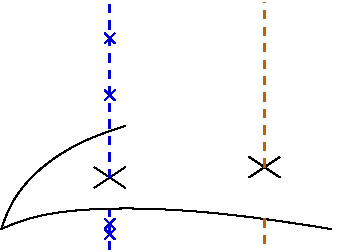
\includegraphics{defor-1.pdf}
\end{picture}%
\setlength{\unitlength}{2171sp}%
\begin{picture}(5059,3666)(279,-1894)
\put(2101,-586){$t=0$}
\put(4351,-511){$t=1$}
\end{picture}%
\end{center}
}
\only<3>{
\begin{center}
\begin{picture}(0,0)%
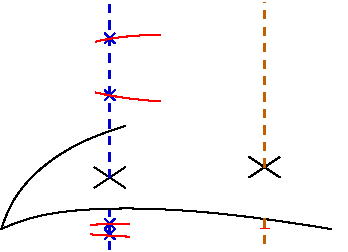
\includegraphics{defor0.pdf}
\end{picture}%
\setlength{\unitlength}{2171sp}%
\begin{picture}(5059,3666)(279,-1894)
\put(2101,-586){$t=0$}
\put(4351,-511){$t=1$}
\end{picture}%
\end{center}
}
\only<4>{
\begin{center}
\begin{picture}(0,0)%
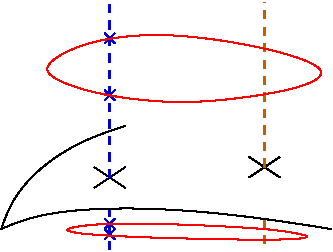
\includegraphics{defor2.pdf}
\end{picture}%
\setlength{\unitlength}{2171sp}%
\begin{picture}(5059,3666)(279,-1894)
\put(2101,-586){$t=0$}
\put(4351,-511){$t=1$}
\end{picture}%
\end{center}
}
\only<5>{
\begin{center}
\begin{picture}(0,0)%
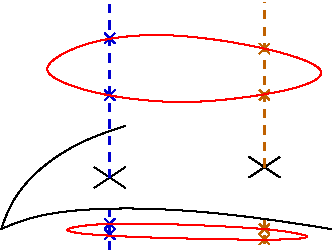
\includegraphics{defor1.pdf}
\end{picture}%
\setlength{\unitlength}{2171sp}%
\begin{picture}(5059,3666)(279,-1894)
\put(2101,-586){$t=0$}
\put(4351,-511){$t=1$}
\end{picture}%
\end{center}
}
\only<6>{
\begin{center}
\begin{picture}(0,0)%
  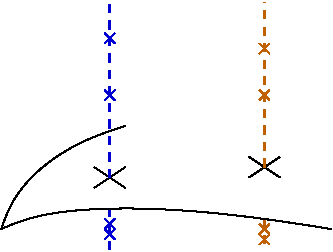
\includegraphics{defor3.pdf}
\end{picture}%
\setlength{\unitlength}{2171sp}%
\begin{picture}(5059,3666)(279,-1894)
\put(2101,-586){$t=0$}
\put(4351,-511){$t=1$}
\end{picture}%
\end{center}
}
\only<1,2>{
\[
\blue{r(T)=0, X_1=v_1(T),\dots,X_n=v_n(T) \text{~in~} \K[T]}
\] 
}
\only<3>{
\[
\red{R(t,T)=0, X_1=V_1(t,T),\dots,X_n=V_n(t,T) \text{~in~} \K[[t]][T]}
\] 
}
\only<4>{
\[
\red{\rho(t,T)=0, X_1=\phi_1(t,T),\dots,X_n=\phi_n(t,T) \text{~in~} \K(t)[T]}
\] 
}
\only<5,6>{
\[
\cd{s(T)=0, X_1=w_1(T),\dots,X_n=w_n(T) \text{~in~} \K[T]}
\] 
}
\end{overlayarea}

\end{frame}

%%%%%%%%%%%%%%%%%%%%%%%%%%%%%%%%%%%%%%%%%%%%%%%%%%%%%%%%%%%%
%%%%%%%%%%%%%%%%%%%%%%%%%%%%%%%%%%%%%%%%%%%%%%%%%%%%%%%%%%%%
%%%%%%%%%%%%%%%%%%%%%%%%%%%%%%%%%%%%%%%%%%%%%%%%%%%%%%%%%%%%

\begin{frame}

\frametitle{Previous work}

\rf{Giusti-Lecerf-Salvy}
\begin{itemize}
\item symbolic Newton iteration
\end{itemize}

\medskip

\rf{Jeronimo {\it et al.}}
\begin{itemize}
\item symbolic polyhedral homotopies 
\end{itemize}

\medskip

\rf{Safey El Din-Schost}
\begin{itemize}
\item bit complexity of multi-homogeneous homotopies
\end{itemize}

\end{frame}

%%%%%%%%%%%%%%%%%%%%%%%%%%%%%%%%%%%%%%%%%%%%%%%%%%%%%%%%%%%%
%%%%%%%%%%%%%%%%%%%%%%%%%%%%%%%%%%%%%%%%%%%%%%%%%%%%%%%%%%%%
%%%%%%%%%%%%%%%%%%%%%%%%%%%%%%%%%%%%%%%%%%%%%%%%%%%%%%%%%%%%

\begin{frame}

\frametitle{Homotopies for non-square systems}

\begin{overlayarea}{\linewidth}{15\baselineskip}

\rk{Assumptions}
\begin{itemize}
\only<2>{\item\textcolor{darkgreen}{all components of $V(\bh) \subset  \Kbar{}^{n+1}$ have dimension at least $1$}}
\only<1,3,4,5>{\item all components of $V(\bh) \subset  \Kbar{}^{n+1}$ have dimension at least $1$}
\only<3>{\item \textcolor{Pink}{if a localization $\bh \cdot \K[t,\bX]_\mathfrak{m}$  has height $n$, it is unmixed}}
\only<1,2,4,5>{\item if a localization $\bh \cdot \K[t,\bX]_\mathfrak{m}$  has height $n$, it is unmixed}
\only<4>{\textcolor{red}{\item  $\bX$-degree($\bb$)=$\bX$-degree($\bh$), with no solution at infinity}}
\only<1,2,3,5>{\item   $\bX$-degree($\bb$)=$\bX$-degree($\bh$), with no solution at infinity}
\item \only<5>{\textcolor{blue}{the ideal generated by $\bb$ is radical}}
\only<1,2,3,4>{the ideal generated by $\bb$ is radical}
\end{itemize}

\medskip

\only<1>{
\mythm{Theorem}{
Let $\kappa$ be the number of solutions of the start system.
\begin{itemize}[leftmargin=1em]
\item target system has at most $\kappa$ solutions (with multiplicities)
\item they can be computed by a symbolic homotopy
\end{itemize}
}
}
\only<2>{\centerline{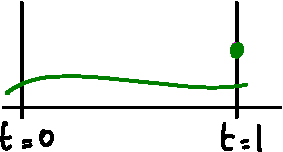
\includegraphics{green-crop.pdf}}}
\only<4>{\centerline{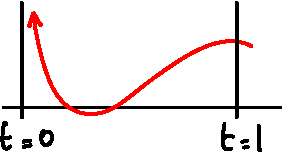
\includegraphics{red-crop.pdf}}}
\only<5>{\centerline{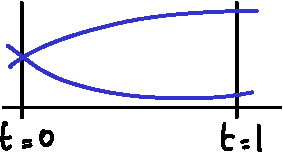
\includegraphics{blue-crop.pdf}}}
\only<3>{\centerline{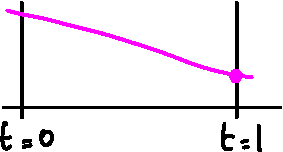
\includegraphics{pink-crop.pdf}}}

\end{overlayarea}

\end{frame}


%%%%%%%%%%%%%%%%%%%%%%%%%%%%%%%%%%%%%%%%%%%%%%%%%%%%%%%%%%%%
%%%%%%%%%%%%%%%%%%%%%%%%%%%%%%%%%%%%%%%%%%%%%%%%%%%%%%%%%%%%
%%%%%%%%%%%%%%%%%%%%%%%%%%%%%%%%%%%%%%%%%%%%%%%%%%%%%%%%%%%%

\begin{frame}

\frametitle{Subroutines}

\rk{Mainly classical} (Newton iteration, rational reconstruction, \dots)

\medskip

\rk{Another ingredient:} local dimension test
\begin{itemize}
\item we are given $\bx$ such that $\bh(\bx)=0$
\item either $\bx$ belongs to a positive-dimensional component of  $V(\bh)$,
 or $\bx$ is isolated with multiplicity at most $\kappa$
\item $\bh$ is given by a straight-line program of length $L$.
\end{itemize}

\mythm{Proposition}{
We can decide whether $\bx$ is an isolated root of $V(\bbf)$ using
\red{$(\kappa\,L\,m)^{O(1)}$} operations in~$\K$.
}

Previous work by \rf{Marinari {\it et al.}}, \rf{Mourrain} and
\rf{Bates {\it et al.}} adapted to our SLP model.

\end{frame}

%%%%%%%%%%%%%%%%%%%%%%%%%%%%%%%%%%%%%%%%%%%%%%%%%%%%%%%%%%%%
%%%%%%%%%%%%%%%%%%%%%%%%%%%%%%%%%%%%%%%%%%%%%%%%%%%%%%%%%%%%
%%%%%%%%%%%%%%%%%%%%%%%%%%%%%%%%%%%%%%%%%%%%%%%%%%%%%%%%%%%%

\begin{frame}

\frametitle{Column degrees (aka the easy case)}

When there are no polynomials $G$ (to simplify), let 
\[
\mH=\begin{bmatrix}
1 & 1 & \cdots & 1 \\
1 & 2 & \cdots & 2^{q-1} \\
\vdots & \vdots & & \vdots \\
1 & p & \cdots & p^{q-1} 
\end{bmatrix}
\begin{bmatrix}
\ell_{1,1} \cdots \ell_{1,\alpha_1}\\
&\ell_{2,1} \cdots \ell_{2,\alpha_2}\\
&&\ddots\\
&&&\ell_{q,1} \cdots \ell_{q,\alpha_q}
\end{bmatrix}
\]
with $\ell_{i,j}$ random linear forms, and $\bh$ be the $p$-minors 
of $(1-t)\mH + t\mF$.

\medskip

\rk{Fact:} $\rank(\mH) < p$ $\iff$ $n$ products $\ell_{i,1} \cdots \ell_{i,\alpha_i}$ vanish

\medskip

This leads us to solve $E_n(\alpha_1,\dots,\alpha_q)$ linear systems of size $n$

\medskip

\rk{Remark:} 
\begin{itemize}
\item $\mH$ already used in \rf{Nie and Ranestad} for degree bounds
\item Lagrange multipliers + bihomogeneous homotopy give similar results
\end{itemize}

\end{frame}


%%%%%%%%%%%%%%%%%%%%%%%%%%%%%%%%%%%%%%%%%%%%%%%%%%%%%%%%%%%%
%%%%%%%%%%%%%%%%%%%%%%%%%%%%%%%%%%%%%%%%%%%%%%%%%%%%%%%%%%%%
%%%%%%%%%%%%%%%%%%%%%%%%%%%%%%%%%%%%%%%%%%%%%%%%%%%%%%%%%%%%

\begin{frame}

\frametitle{Row degrees (aka the useful case)}

\begin{overlayarea}{\linewidth}{15\baselineskip}

Let 
\[
\mH=\begin{bmatrix}
\only<1>{{L_{1,1}}}\only<2,3,4,5,6>{\red{L_{1,1}}} &  &  && \only<1,2>{L_{1,p+1}}\only<3,4,5,6>{\red{L_{1,p+1}}} & \cdots & \only<1,2>{L_{1,q}}\only<3,4,5,6>{\red{L_{1,q}}} \\
 & \only<1>{{L_{2,2}}}\only<2,3,4,5,6>{\red{L_{2,2}}}  &  &&  \only<1,2>{L_{2,p+1}}\only<3,4,5,6>{\red{L_{2,p+1}}} & \cdots & \only<1,2>{L_{2,q}}\only<3,4,5,6>{\red{L_{2,q}}} \\
 &  & \ddots& & \vdots && \vdots \\
 &  & &   L_{p,p} &  L_{p,p+1} & \cdots & L_{p,q} \\
\end{bmatrix}
\]
with $L_{i,j}$ a product of $\beta_i$ random linear forms,
and $\bh$ as before.

\medskip

\begin{tabular}{lcl}
\hspace{-0.6em}\rk{Fact:} $\rank(\mH)< p$\hspace{-0.8em} &$\iff$& \hspace{-0.9em} some (say $\tau$)
of the $L_{i,i}$ vanish and \\
&& \only<3,4,5,6>{\hspace{-0.9em} the corresponding right-block is rank-deficient}\\
&& \only<4,5,6>{\hspace{-1.2em} $\implies$ $\tau \times (n-1)$ matrix in $n-\tau$ variables}
\end{tabular}

\medskip

\only<5,6>{\rk{Theorem:} for generic $L_{i,j}$, the homotopy works}

\medskip 

\only<6>{\rk{Caveat:} We recursively use a homotopy to solve the start system

}

\end{overlayarea}

\end{frame}

%%%%%%%%%%%%%%%%%%%%%%%%%%%%%%%%%%%%%%%%%%%%%%%%%%%%%%%%%%%%
%%%%%%%%%%%%%%%%%%%%%%%%%%%%%%%%%%%%%%%%%%%%%%%%%%%%%%%%%%%%
%%%%%%%%%%%%%%%%%%%%%%%%%%%%%%%%%%%%%%%%%%%%%%%%%%%%%%%%%%%%

\begin{frame}

\frametitle{Conclusions}

\rk{Done}
\begin{itemize}
\item symbolic algorithm, complexity
\item prototype
\end{itemize}

\medskip

\rk{To do}
\begin{itemize}
\item error probability 
\item bit complexity
\item numerical version
\item higher rank defect
\end{itemize}

\end{frame}

\end{document}

